% ============================================================
%  Chapitre 8 : Déploiement — Intégration du système RAG dans AutoMoni
% ============================================================

% Définition du langage JavaScript pour le package listings
\lstdefinelanguage{JavaScript}{
  keywords={const, let, var, function, return, if, else, for, while,
            true, false, null, undefined, new, this, async, await,
            typeof, module, exports, require, process},
  morestring=[b]',
  morestring=[b]",
  morecomment=[l]{//},
  morecomment=[s]{/*}{*/},
  sensitive=true,
}

\chapter{Déploiement}
\section*{Introduction}
% ─────────────────────────────────────────────────────────────
La phase de déploiement constitue l’aboutissement des travaux de modélisation et leur transition vers une utilisation concrète par les utilisateurs finaux. Après les étapes de conception, d’optimisation et de validation du pipeline RAG, l’objectif est désormais de rendre la solution opérationnelle au sein d’un environnement applicatif réel.

Dans le cadre de ce projet, la mise en production repose sur deux composantes principales : d’une part, le \textbf{système RAG} développé en Python et exposé sous forme d’API REST à l’aide de FastAPI, et d’autre part, l’\textbf{application web AutoMoni}, une plateforme de monitoring SAP développée avec SAP CAP et React, au sein de laquelle le chatbot intelligent a été intégré.

Ce chapitre présente l’architecture générale de déploiement, les différentes étapes de mise en service des composants, le mécanisme d’intégration du chatbot dans l’interface applicative, ainsi qu’une présentation de l’interface utilisateur finale. Il se conclut par une évaluation des performances du système à travers un benchmark comparatif.
% ─────────────────────────────────────────────────────────────
\section{Architecture globale de déploiement}
% ─────────────────────────────────────────────────────────────

\subsection{Vue d'ensemble}

Le système déployé repose sur une architecture à trois couches distinctes communiquant via des interfaces bien définies. La figure 8.2  illustre l'ensemble des composants et leurs interconnexions.

% Required in preamble:
% \usetikzlibrary{arrows.meta, fit, backgrounds, shadows.blur, calc}

% Preamble: \usetikzlibrary{arrows.meta, fit, backgrounds, shadows.blur, calc}

\begin{figure}[H]
\centering
\resizebox{0.97\textwidth}{!}{%
\begin{tikzpicture}[
  font=\small,
  %% ── Box style ───────────────────────────────────────────
  box/.style={
    draw=#1, rectangle, rounded corners=6pt,
    minimum width=3.3cm, minimum height=1.4cm,
    text centered, align=center, font=\footnotesize,
    fill=white, line width=1.1pt,
    blur shadow={shadow blur steps=4, shadow xshift=1.5pt,
                 shadow yshift=-1.5pt, shadow blur radius=3pt,
                 shadow opacity=0.15}
  },
  box/.default=black,
  %% ── Arrow styles ────────────────────────────────────────
  arr/.style={-{Stealth[length=7pt,width=5pt]}, line width=1.2pt, #1},
  arr/.default=black,
  arrbi/.style={
    {Stealth[length=6pt,width=4pt]}-{Stealth[length=6pt,width=4pt]},
    line width=1.0pt, #1},
  arrbi/.default=black,
  %% ── Label styles ────────────────────────────────────────
  lbl/.style={font=\scriptsize\ttfamily, fill=white, inner sep=2.5pt,
              rounded corners=3pt, draw=gray!35, line width=0.6pt},
  ilbl/.style={font=\tiny\sffamily, fill=white, inner sep=1.5pt,
               rounded corners=2pt, draw=gray!25, line width=0.5pt},
  portbadge/.style={
    font=\tiny\bfseries\ttfamily, fill=white,
    draw=#1, rounded corners=3pt,
    inner sep=2.5pt, text=#1, line width=0.8pt},
  portbadge/.default=black,
  %% ── Layer title style ───────────────────────────────────
  layertitle/.style={
    font=\footnotesize\bfseries, text=#1,
    fill=white, draw=#1, rounded corners=4pt,
    inner xsep=8pt, inner ysep=4pt, line width=0.9pt},
  layertitle/.default=black,
]

%% ════════════════════════════════════════════════════════════
%% LAYER 1 BOXES — Frontend  (y = 8.0)
%% ════════════════════════════════════════════════════════════
\node[box=SAPBlue] (shell)    at (-5.5, 8.0)
  {{\color{SAPBlue}\textbf{ShellBar}}\\[2pt]\scriptsize Bouton IA};
\node[box=SAPBlue] (panel)    at (-1.7, 8.0)
  {{\color{SAPBlue}\textbf{ChatPanel}}\\[2pt]\scriptsize Tiroir latéral};
\node[box=SAPBlue] (chatpage) at ( 2.0, 8.0)
  {{\color{SAPBlue}\textbf{Chatbot.jsx}}\\[2pt]\scriptsize Page dédiée};
\node[box=SAPBlue] (pages)    at ( 5.8, 8.0)
  {{\color{SAPBlue}\textbf{25+ Pages}}\\[2pt]\scriptsize Monitoring};

%% ════════════════════════════════════════════════════════════
%% LAYER 2 BOXES — CAP / Métier  (y = 4.5)
%% ════════════════════════════════════════════════════════════
\node[box=SAPGreen] (chatSrv) at (-3.5, 4.5)
  {{\color{SAPGreen}\textbf{chat-service}}\\[2pt]\scriptsize OData Action};
\node[box=SAPGreen] (monSrv)  at ( 1.0, 4.5)
  {{\color{SAPGreen}\textbf{monitoring-service}}\\[2pt]\scriptsize 18 entités OData};
\node[box=SAPGreen] (mongo)   at ( 5.3, 4.5)
  {{\color{SAPGreen}\textbf{MongoDB Atlas}}\\[2pt]\scriptsize Données monitoring};

%% ════════════════════════════════════════════════════════════
%% LAYER 3 BOXES — RAG / Python  (y = 1.0)
%% ════════════════════════════════════════════════════════════
\node[box=SAPOrange] (api)    at (-5.5, 1.0)
  {{\color{SAPOrange}\textbf{api.py}}\\[2pt]\scriptsize FastAPI};
\node[box=SAPOrange] (pipe)   at (-1.7, 1.0)
  {{\color{SAPOrange}\textbf{rag\_pipeline v2}}\\[2pt]\scriptsize Pipeline RAG};
\node[box=SAPOrange] (ollama) at ( 2.0, 1.0)
  {{\color{SAPOrange}\textbf{Ollama}}\\[2pt]\scriptsize llama3.2:3b};
\node[box=SAPOrange] (pg)     at ( 5.8, 1.0)
  {{\color{SAPOrange}\textbf{PostgreSQL}}\\[2pt]\scriptsize pgvector};

%% ════════════════════════════════════════════════════════════
%% BACKGROUND BANDS  (fit snugly around boxes only)
%% ════════════════════════════════════════════════════════════
\begin{scope}[on background layer]
  \node[draw=SAPBlue,   fill=SAPLightBlue,   rounded corners=10pt,
        inner sep=12pt, line width=1.3pt,
        fit=(shell)(panel)(chatpage)(pages)]   (layer1) {};
  \node[draw=SAPGreen,  fill=SAPLightGreen,  rounded corners=10pt,
        inner sep=12pt, line width=1.3pt,
        fit=(chatSrv)(monSrv)(mongo)]          (layer2) {};
  \node[draw=SAPOrange, fill=SAPLightOrange, rounded corners=10pt,
        inner sep=12pt, line width=1.3pt,
        fit=(api)(pipe)(ollama)(pg)]           (layer3) {};
\end{scope}

%% ════════════════════════════════════════════════════════════
%% LAYER TITLE BANNERS — placed ABOVE each band (no overlap)
%% ════════════════════════════════════════════════════════════
\node[layertitle=SAPBlue, anchor=south west]
  at ([xshift=6pt, yshift=3pt]layer1.north west)
  {Couche Présentation — Frontend React / SAP UI5};
\node[portbadge=SAPBlue, anchor=south east]
  at ([xshift=-6pt, yshift=3pt]layer1.north east)
  {:3000};

\node[layertitle=SAPGreen, anchor=south west]
  at ([xshift=6pt, yshift=3pt]layer2.north west)
  {Couche Métier — SAP CAP / Express};
\node[portbadge=SAPGreen, anchor=south east]
  at ([xshift=-6pt, yshift=3pt]layer2.north east)
  {:4004};

\node[layertitle=SAPOrange, anchor=south west]
  at ([xshift=6pt, yshift=3pt]layer3.north west)
  {Couche RAG — Python / FastAPI};
\node[portbadge=SAPOrange, anchor=south east]
  at ([xshift=-6pt, yshift=3pt]layer3.north east)
  {:8000};

%% ════════════════════════════════════════════════════════════
%% INTER-LAYER ARROWS
%% ════════════════════════════════════════════════════════════

%% ChatPanel → chat-service  (primary, solid)
\draw[arr=SAPBlue!80]
  (panel.south) -- ++(0,-0.75)
  node[lbl, pos=0.6, right=4pt]{\texttt{POST /odata/v4/chat/query}}
  -| (chatSrv.north);

%% Chatbot.jsx → chat-service  (secondary, dashed)
\draw[arr=SAPBlue!35, dashed, line width=0.85pt]
  (chatpage.south) -- ++(0,-1.3) -| (chatSrv.north);

%% 25+Pages → monitoring-service  (secondary, dashed)
\draw[arr=SAPBlue!35, dashed, line width=0.85pt]
  (pages.south) -- ++(0,-1.3) -| (monSrv.north);

%% chat-service → api.py  (RAG call)
\draw[arr=SAPGreen!80]
  (chatSrv.south) -- ++(0,-0.75)
  node[lbl, pos=0.6, right=4pt]{\texttt{POST http://localhost:8000/query}}
  -| (api.north);

%% ════════════════════════════════════════════════════════════
%% INTRA-LAYER ARROWS — RAG layer
%% (labels placed BELOW the connecting line to avoid box overlap)
%% ════════════════════════════════════════════════════════════
\draw[arrbi=SAPOrange]
  (api.east) -- node[ilbl, below=3pt]{embed + retrieve} (pipe.west);

\draw[arrbi=SAPOrange]
  (pipe.east) -- node[ilbl, below=3pt]{prompt} (ollama.west);

%% pipe → PostgreSQL: routed below to avoid crossing Ollama
\draw[arr=SAPOrange]
  (pipe.south) -- ++(0,-0.55)
  -- node[ilbl, below=2pt]{vecteurs}
     ($(pg.south)+(0,-0.55)$)
  -- (pg.south);

%% ════════════════════════════════════════════════════════════
%% INTRA-LAYER ARROWS — CAP layer
%% ════════════════════════════════════════════════════════════
\draw[arrbi=SAPGreen]
  (monSrv.east) -- node[ilbl, above=2pt]{CRUD} (mongo.west);

%% ════════════════════════════════════════════════════════════
%% RIGHT-SIDE DATA-FLOW SPINE
%% ════════════════════════════════════════════════════════════
\coordinate (spineTop) at (9.0, 8.8);
\coordinate (spineMid) at (9.0, 5.2);
\coordinate (spineBot) at (9.0, 1.7);

\draw[arr=gray!45, line width=0.9pt, dashed]
  (spineTop) -- (spineMid)
  node[midway, right=3pt, font=\tiny\sffamily\color{gray!65}, align=center]
    {Requête\\utilisateur};

\draw[arr=gray!45, line width=0.9pt, dashed]
  (spineMid) -- (spineBot)
  node[midway, right=3pt, font=\tiny\sffamily\color{gray!65}, align=center]
    {Inférence\\RAG};

%% ════════════════════════════════════════════════════════════
%% BOTTOM LEGEND
%% ════════════════════════════════════════════════════════════
\begin{scope}[shift={(0,-0.55)}]
  \draw[arr=gray!70, line width=1.0pt]
    (-6.5,-0.05) -- (-5.1,-0.05);
  \node[right, font=\tiny\sffamily\color{gray!60}] at (-5.0,-0.05)
    {Appel synchrone};

  \draw[arr=gray!50, dashed, line width=0.85pt]
    (-2.5,-0.05) -- (-1.1,-0.05);
  \node[right, font=\tiny\sffamily\color{gray!60}] at (-1.0,-0.05)
    {Flux secondaire};

  \draw[arrbi=gray!60, line width=0.9pt]
    (1.6,-0.05) -- (3.0,-0.05);
  \node[right, font=\tiny\sffamily\color{gray!60}] at (3.1,-0.05)
    {Échange interne bidirectionnel};
\end{scope}

\end{tikzpicture}%
}
\caption[Architecture de déploiement AutoMoni]{Architecture globale de déploiement du système RAG intégré dans AutoMoni}
\label{fig:deploy_arch}
\end{figure}

\section{Diagramme de cas d'utilisation général}

Dans cette section, les exigences fonctionnelles du système déployé sont représentées à l'aide d'un diagramme de cas d'utilisation conforme au langage de modélisation UML. Ce diagramme (voir figure~\ref{fig:usecase_deploy}) met en évidence les différents acteurs du système ainsi que les interactions possibles entre ces acteurs et les fonctionnalités offertes par l'application. Il permet ainsi de fournir une vision globale du comportement du système et des services qu'il propose aux utilisateurs.

\begin{figure}[H]
    \centering
    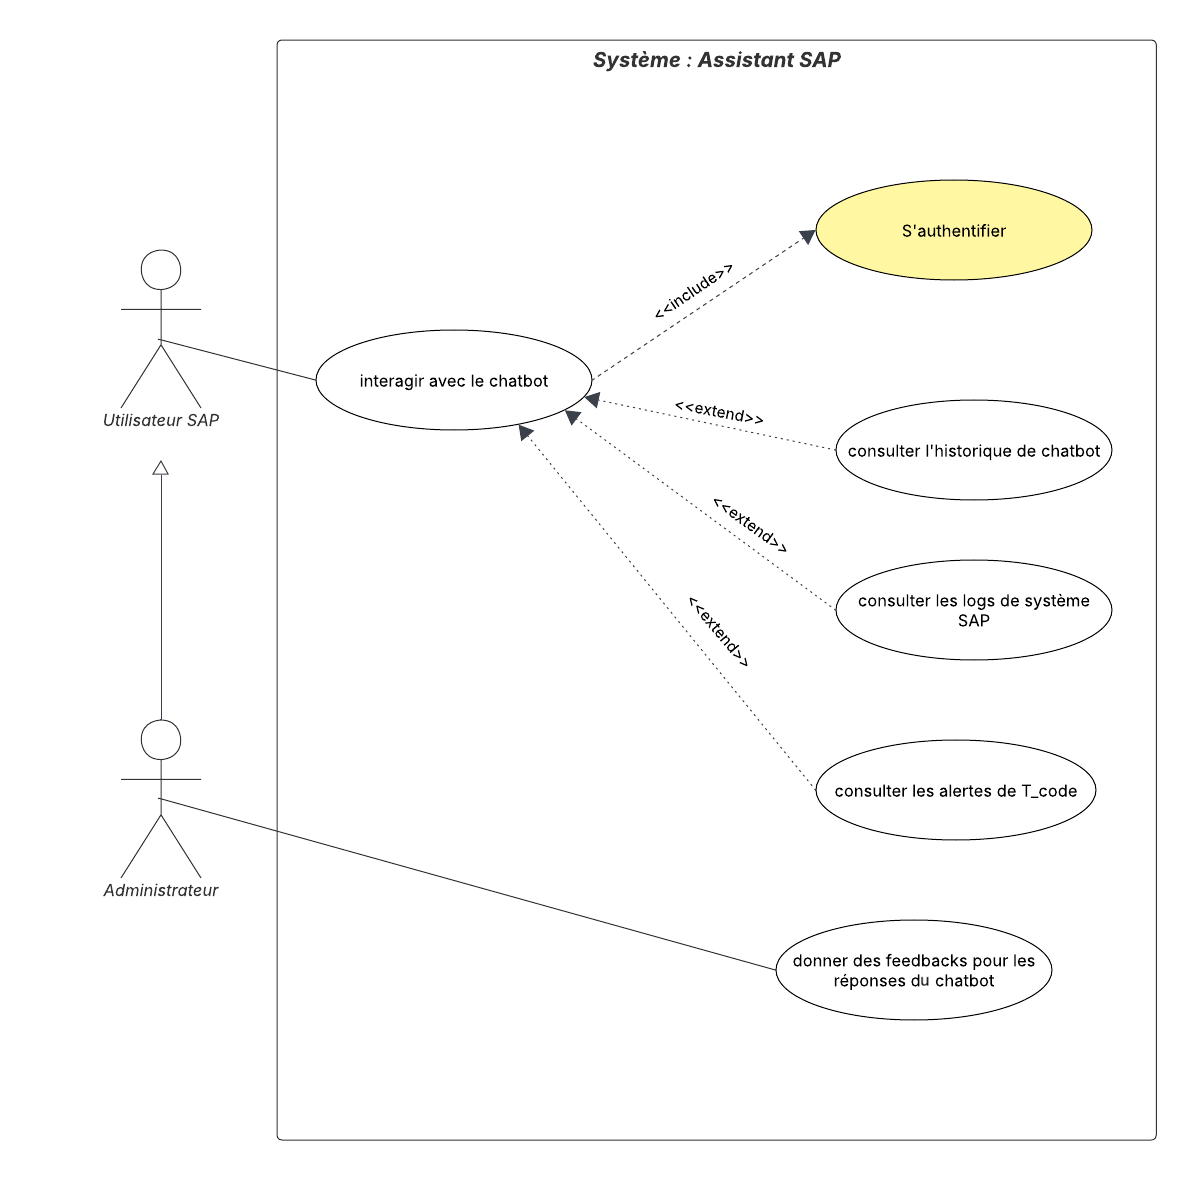
\includegraphics[width=0.9\textwidth]{images/casutilisation.png}
    \caption[Diagramme de cas d'utilisation]{Diagramme de cas d'utilisation général du système déployé}
    \label{fig:usecase_deploy}
\end{figure}

\subsection{Technologies utilisées}

L'ensemble de la pile technologique mise en œuvre est résumé dans le tableau~\ref{tab:tech_stack}.

\begin{table}[H]
\centering
\caption{Pile technologique du système déployé}
\label{tab:tech_stack}
\begin{tabularx}{\textwidth}{|l|l|X|}
\hline
\textbf{Couche} & \textbf{Technologie} & \textbf{Rôle} \\
\hline
Frontend & React 19 + SAP UI5 Web Components & Interface utilisateur, affichage du chatbot \\
\hline
Backend & SAP CAP v8 + Express.js & Services OData, proxy vers l'API RAG (port 4004) \\
\hline
Base de données & MongoDB Atlas & Stockage des données de monitoring SAP (18 collections) \\
\hline
API RAG & FastAPI + Uvicorn & Exposition du pipeline RAG en REST (port 8000) \\
\hline
LLM & Ollama (llama3.2:3b / qwen2.5:7b) & Génération locale des réponses (port 11434) \\
\hline
Embeddings & BAAI/bge-large-en-v1.5 & Vectorisation des requêtes et des documents \\
\hline
Base vectorielle & PostgreSQL + pgvector & Stockage et recherche hybride (port 5432) \\
\hline
\end{tabularx}
\end{table}


% ─────────────────────────────────────────────────────────────────────────────

% ─────────────────────────────────────────────────────────────
\section{Déploiement du système RAG}
% ─────────────────────────────────────────────────────────────

\subsection{Configuration de l'environnement}

Le système RAG est configuré à travers un fichier \texttt{.env} qui centralise les paramètres d'accès aux services externes. Les trois variables essentielles sont la chaîne de connexion à la base de données PostgreSQL, et les noms des modèles LLM disponibles via Ollama

\subsection{Infrastructure de la base de données vectorielle}

\begin{lstlisting}[language=SQL, caption={Création de l'index vectoriel HNSW sur la table sap\_chunks}]
CREATE INDEX sap_chunks_hnsw ON sap_chunks
    USING hnsw (embedding vector_cosine_ops)
    WITH (m = 16, ef_construction = 64);
\end{lstlisting}

% ─────────────────────────────────────────────────────────────
\subsection{Schéma de la base de données PostgreSQL}
\label{subsec:schema_bdd}
% ─────────────────────────────────────────────────────────────

La base de données PostgreSQL du système héberge \textbf{21 tables} organisées en quatre
groupes fonctionnels, chacun correspondant à un rôle distinct dans l'architecture RAG déployée~:

\begin{itemize}[leftmargin=2em]
  \item \textbf{Tables fondamentales RAG/CAG~:} \texttt{sap\_chunks} (76~463 vecteurs de
        dimension 1~024, index HNSW cosinus) et \texttt{qa\_cache} (cache sémantique des
        réponses générées avec leurs embeddings de requête).
  \item \textbf{Tables d'interaction utilisateur~:} \texttt{conversations} (historique de
        dialogue multi-tours avec détection d'intention et réécriture de requête) et
        \texttt{admin\_feedback} (notations et corrections humaines avec vecteur de la
        question originale pour invalidation du cache).
  \item \textbf{Tables de monitoring SAP~:} 12~tables alimentées en continu via PyRFC,
        correspondant aux T-codes de supervision~: SM37, SM51, SM66, SM12, SM13, SM58,
        SMQ1, SOST, SP01, ST03N, ST13, ST22.
  \item \textbf{Tables de métriques système~:} 5~tables de métriques OS et base de données
        (\texttt{cpu}, \texttt{memory}, \texttt{fsys}, \texttt{db02}, \texttt{mss\_db}).
\end{itemize}

La figure~\ref{fig:class_core} présente le diagramme de classes détaillé des quatre tables
fondamentales avec l'ensemble de leurs attributs et les associations logiques entre elles.
La figure~\ref{fig:class_monitoring} présente les 17~tables de monitoring et de métriques dans
un format compact.

\begin{figure}[H]
\centering
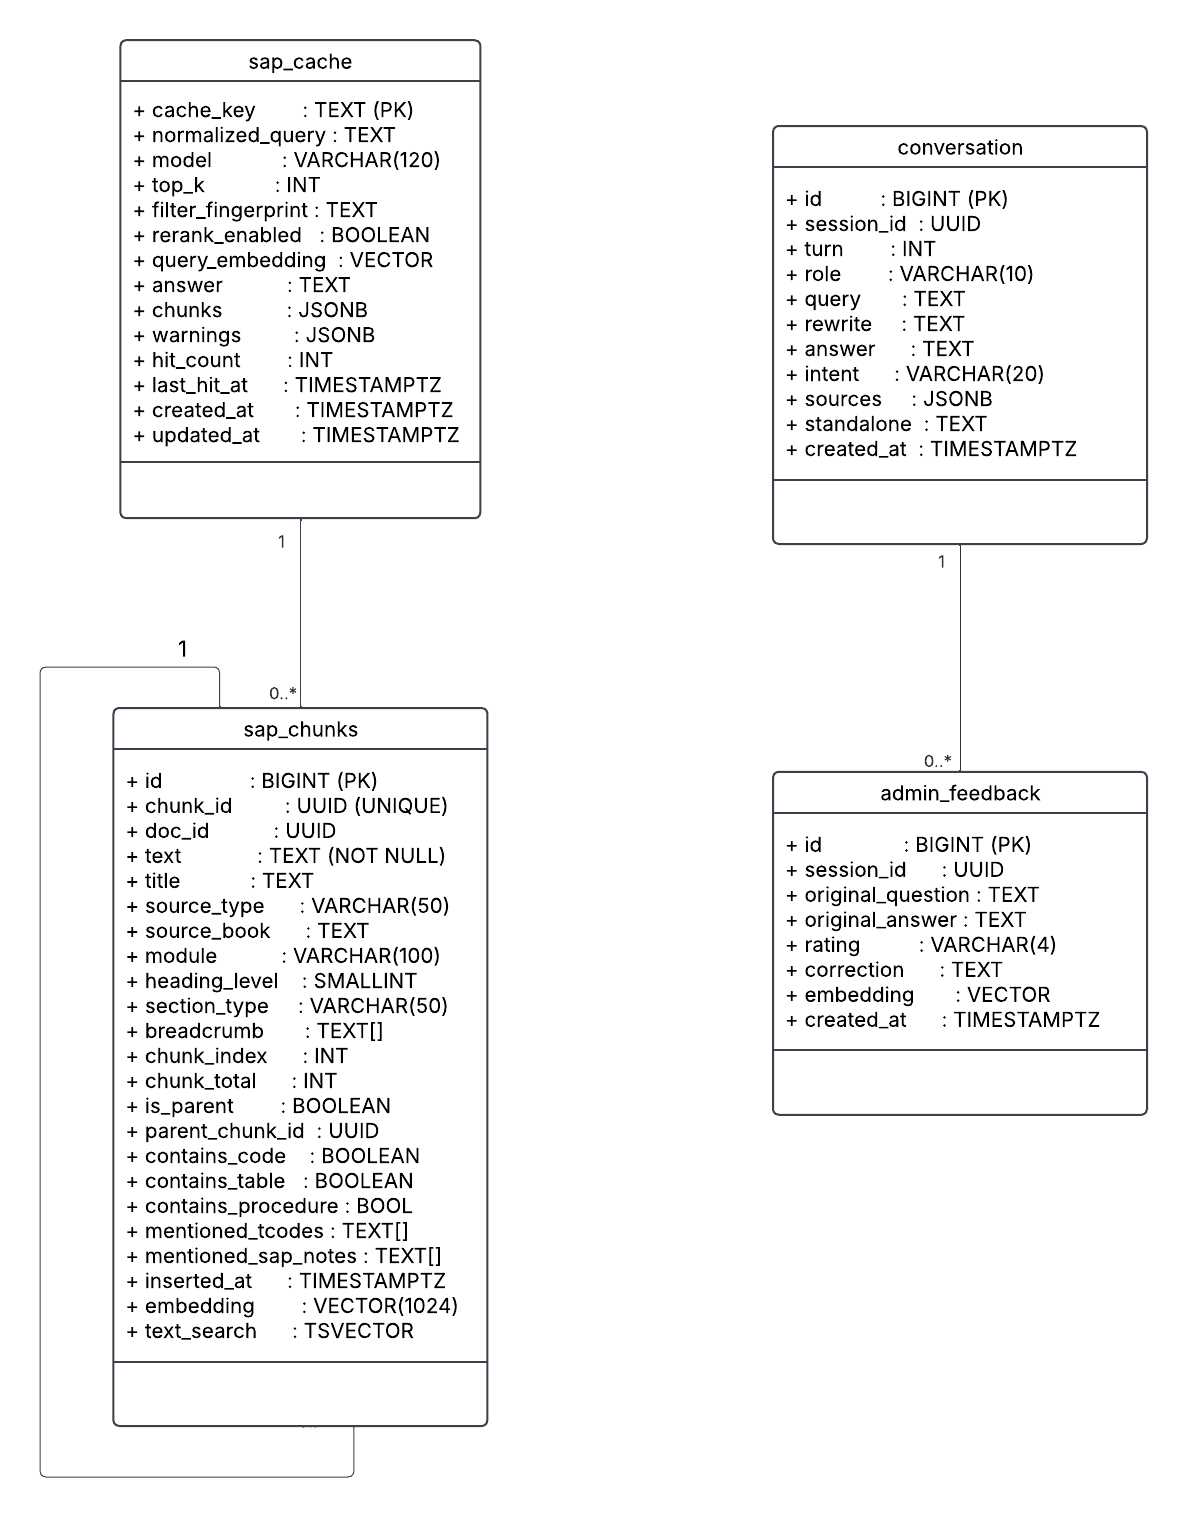
\includegraphics[width=0.90\textwidth]{images/Blank diagram.png}
\caption[Diagramme de classes (PostgreSQL)]{Diagramme de classes --- Tables fondamentales du système RAG (PostgreSQL)}
\label{fig:class_core}
\end{figure}


\subsection{Démarrage de l'API FastAPI}

Le serveur FastAPI est lancé via \textbf{Uvicorn}, le serveur ASGI de référence pour les applications Python asynchrones~:

\begin{lstlisting}[language=sh, caption={Commande de démarrage de l'API RAG}]
cd C:\Users\Youss\Documents\RAG_SAP\rag
uvicorn api:app --host 0.0.0.0 --port 8000 --reload
\end{lstlisting}

\subsection{Endpoints REST exposés}

L'API FastAPI expose trois endpoints documentés automatiquement via Swagger UI (\texttt{http://localhost:8000/docs})~:

\begin{table}[H]
\centering
\caption{Endpoints de l'API RAG (api.py)}
\label{tab:api_endpoints}
\begin{tabularx}{\textwidth}{|l|l|X|}
\hline
\textbf{Méthode} & \textbf{Endpoint} & \textbf{Description} \\
\hline
\texttt{POST} & \texttt{/query} & Reçoit une question et un session\_id, exécute le pipeline RAG, renvoie la réponse avec sources et avertissements \\
\hline
\texttt{DELETE} & \texttt{/session/\{session\_id\}} & Supprime l'historique de conversation associé à une session \\
\hline
\texttt{GET} & \texttt{/health} & Vérifie la disponibilité du service et retourne le modèle actif \\
\hline
\end{tabularx}
\end{table}

Le corps de la requête \texttt{POST /query} accepte les paramètres suivants~:

\begin{lstlisting}[language=Python, caption={Schéma de la requête POST /query (api.py)}]
class QueryRequest(BaseModel):
    question:      str
    session_id:    str = ""
    top_k:         int = TOP_K          # defaut : 5
    model:         str = OLLAMA_MODEL   # defaut : llama3.2:3b
    filter_tcode:  Optional[str] = None
    filter_module: Optional[str] = None
    filter_source: Optional[str] = None
\end{lstlisting}

\begin{figure}[H]
\centering
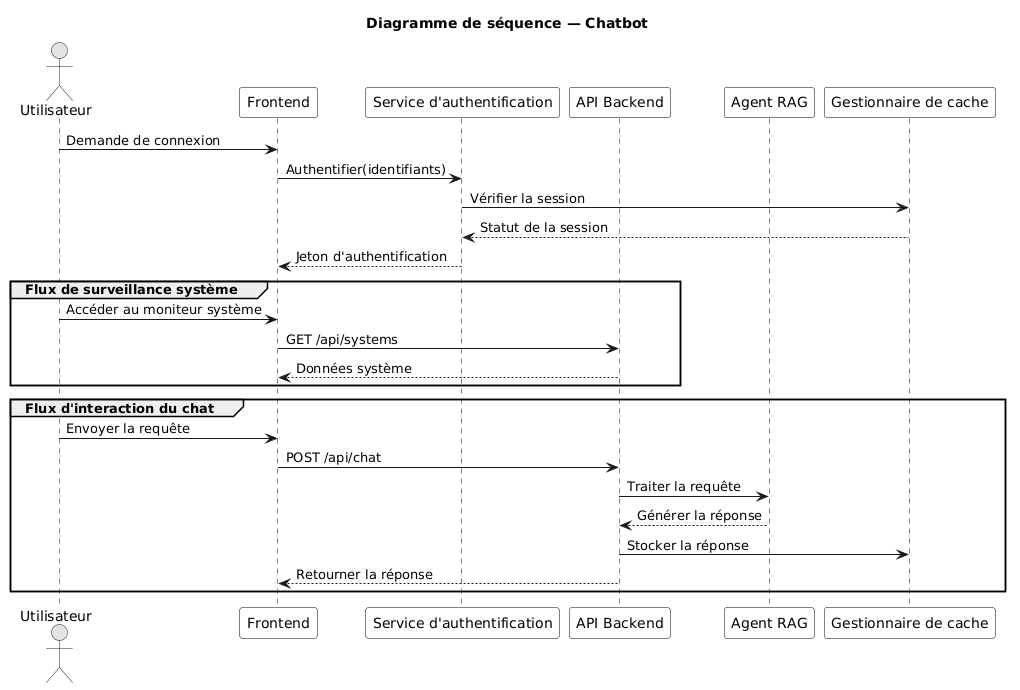
\includegraphics[width=\textwidth]{images/sequence_chatbot_fr.png}
\caption[Diagramme de séquence — interaction complète]{Diagramme de séquence  cycles complets d'interaction~: initialisation de session, surveillance SAP et chatbot RAG}
\label{fig:sequence_requete}
\end{figure}

\subsection{Paramètres clés du pipeline}

Le tableau~\ref{tab:pipeline_params} regroupe les hyperparamètres déterminants du pipeline RAG déployé en production~:

\begin{table}[H]
\centering
\caption{Paramètres de configuration du pipeline RAG (rag\_pipeline.py)}
\label{tab:pipeline_params}
\begin{tabularx}{\textwidth}{|l|l|X|}
\hline
\textbf{Paramètre} & \textbf{Valeur} & \textbf{Rôle} \\
\hline
\texttt{FETCH\_K} & 15 & Nombre de candidats récupérés par recherche vectorielle \\
\hline
\texttt{RERANK\_K} & 10 & Nombre de candidats transmis au cross-encoder après RRF \\
\hline
\texttt{TOP\_K} & 5 & Nombre final de chunks injectés dans le prompt LLM \\
\hline
\texttt{CAG\_MAX\_CHUNKS} & 3 & Chunks pré-chargés max pour les requêtes T-code (CAG) \\
\hline
\texttt{MIN\_SCORE} & 0.05 / 0.30 & Seuil minimal de similarité cosinus (adaptatif selon l'intention) \\
\hline
\texttt{MIN\_RERANK\_SCORE} & 2.0 & Seuil de rejet par le cross-encoder (échelle $-10$ à $+10$) \\
\hline
\texttt{MAX\_CHUNKS\_PER\_SOURCE} & 3 & Déduplication : maximum de chunks par source \\
\hline
$W_{\text{vec}}$ / $W_{\text{BM25}}$ & 0.4 / 0.6 & Poids de fusion RRF (BM25 privilégié pour corpus SAP) \\
\hline
\texttt{NUM\_CTX} & 4~096 & Fenêtre de contexte du LLM Ollama (en tokens) \\
\hline
\texttt{Temperature} & 0.1 & Température de génération (réponses déterministes) \\
\hline
\end{tabularx}
\end{table}

% ─────────────────────────────────────────────────────────────
\section{Intégration du chatbot dans l'application web}
% ─────────────────────────────────────────────────────────────

\subsection{Vue d'ensemble de l'intégration}

L'intégration du chatbot dans AutoMoni a été réalisée selon une architecture en trois niveaux~: la \textbf{définition du service} en CDS (Core Data Services), l'\textbf{implémentation du handler} en JavaScript côté CAP, et les \textbf{composants React} côté frontend.

% ── PLACEHOLDER 3 ────────────────────────────────────────────────────────────
% Diagramme à réaliser : architecture des composants de l'intégration chatbot
% Composants : ChatPanel.jsx, AppShell.jsx, chat-service.cds, chat-service.js, api.py
% Suggestions : diagramme de composants UML ou schéma bloc en draw.io

% ─────────────────────────────────────────────────────────────────────────────

\subsection{Définition du service OData (CAP CDS)}

Le service de chatbot est défini dans le fichier \texttt{chat-service.cds} à l'aide du langage CDS de SAP. Il expose une action OData qui accepte la question de l'utilisateur et un identifiant de session, et retourne la réponse structurée du système RAG~:

\begin{lstlisting}[language=SQL, caption={Définition du service chatbot en CDS (chat-service.cds)}]
service ChatService {
  action query(question: String, session_id: String) returns {
    answer:     String;
    sources:    array of String;
    warnings:   array of String;
    session_id: String;
  };
}
\end{lstlisting}

Cette définition génère automatiquement l'endpoint OData \texttt{POST /odata/v4/chat/query}, documenté et typé, directement accessible depuis le frontend React.



\subsection{Composants React du chatbot}

Le chatbot est implémenté côté frontend sous deux formes complémentaires~:

\begin{itemize}[leftmargin=2em]
  \item \textbf{Page dédiée} (\texttt{/chatbot})~: le composant \texttt{Chatbot.jsx} (515 lignes) offre une interface complète avec historique de conversations organisées en sessions, liste des conversations précédentes, zone de réponse avec rendu Markdown via \texttt{react-markdown}, et boutons d'action (nouvelle conversation, effacement).

  \item \textbf{ChatPanel — Tiroir latéral}~: exporté depuis \texttt{Chatbot.jsx}, ce panneau coulissant est intégré dans le composant \texttt{AppShell.jsx} et rendu accessible depuis toutes les pages de l'application via le bouton IA dans la \texttt{ShellBar}. Il est monté paresseusement (\textit{lazy mount}) à la première ouverture afin d'éviter un flash CSS indésirable~:

\begin{lstlisting}[language=JavaScript, caption={Montage paresseux du ChatPanel dans AppShell.jsx}]
const [isChatOpen,    setIsChatOpen]    = useState(false)
const [chatHasOpened, setChatHasOpened] = useState(false)

const onChatbotClick = () => {
  if (!chatHasOpened) setChatHasOpened(true)
  setIsChatOpen(prev => !prev)
}

{chatHasOpened && (
  <ChatPanel open={isChatOpen} onClose={() => setIsChatOpen(false)} />
)}
\end{lstlisting}
\end{itemize}

\subsection{Chatbot et évaluation intégrée en temps réel}
\label{subsec:chatbot-eval}

L'intégration du pipeline d'évaluation directement dans la boucle de traitement du chatbot constitue un apport majeur par rapport à une évaluation \textit{offline} classique. Plutôt que d'utiliser un juge LLM coûteux à chaque appel (comme G-Eval), le système repose sur deux mécanismes complémentaires déclenchés automatiquement à chaque réponse~:

\begin{enumerate}[leftmargin=2em]
  \item \textbf{Détection déterministe des hallucinations}~: la fonction \texttt{check\_hallucinations()} analyse la réponse générée à la recherche de T-codes SAP et de numéros de notes SAP qui ne figurent pas dans les chunks récupérés. Toute mention identifiée comme non ancrée dans les sources est supprimée par \texttt{sanitize\_answer()} avant renvoi à l'utilisateur. Ce mécanisme s'exécute en moins d'une milliseconde sans appel LLM supplémentaire.

  \item \textbf{Attribution des sources}~: les chunks utilisés pour construire la réponse sont retournés dans le champ \texttt{sources} de la réponse JSON, sous forme de références structurées (\textit{«~titre du livre $>$ section~»}).
\end{enumerate}

Ces deux informations sont remontées dans l'interface utilisateur via le contrat d'API défini dans \texttt{chat-service.cds}~:

\begin{lstlisting}[language=SQL, caption={Champs d'évaluation retournés par le service RAG}]
returns {
  answer:   String;          -- reponse nettoyee
  sources:  array of String; -- references des chunks utilises
  warnings: array of String; -- hallucinations detectees et supprimees
  session_id: String;
}
\end{lstlisting}

Le composant React \texttt{BotMessageContent} interprète ces champs et affiche, sous chaque réponse du bot, un indicateur de qualité et la liste des sources consultées~:

\begin{itemize}[leftmargin=2em]
  \item \textbf{Badge vert «~\checkmark~Réponse vérifiée~»}~: aucun avertissement détecté, la réponse est intégralement ancrée dans les sources récupérées.
  \item \textbf{Badge orange «~$\triangle$~N avertissement(s)~»}~: au moins une affirmation a été filtrée pour risque d'hallucination, l'utilisateur est averti.
  \item \textbf{Section «~Sources~» dépliable}~: liste des références documentaires utilisées, permettant à l'utilisateur de vérifier l'origine de chaque information.
\end{itemize}

\begin{lstlisting}[language=JavaScript, caption={Rendu du badge qualité et des sources dans BotMessageContent (Chatbot.jsx)}]
const BotMessageContent = ({ message }) => (
  <>
    <Markdown>{message.text}</Markdown>
    {(message.sources?.length > 0 || message.warnings?.length > 0) && (
      <div className="ag-eval-footer">
        <span className={`ag-quality-badge ${
          message.warnings?.length > 0
            ? 'ag-quality-badge--warn'
            : 'ag-quality-badge--ok'
        }`}>
          {message.warnings?.length > 0
            ? `Warning: ${message.warnings.length} hallucination(s) filtered`
            : 'Response verified'}
        </span>
        <details className="ag-sources">
          <summary>{message.sources.length} source(s)</summary>
          <ul>{message.sources.map((src, i) => <li key={i}>{src}</li>)}</ul>
        </details>
      </div>
    )}
  </>
)
\end{lstlisting}

Cette approche est délibérément \textbf{déterministe et légère}~: contrairement à RAGAS ou G-Eval qui nécessitent un second appel LLM pour scorer la réponse, la détection par règles (T-codes, numéros de notes) est instantanée et 100\,\% reproductible. Elle constitue un mécanisme de premier niveau suffisant pour alerter l'utilisateur sur les cas les plus risqués, RAGAS étant réservé à l'évaluation \textit{offline} en batch du pipeline.

\subsection{Intelligence de navigation — T-codes vers pages monitoring}

Une fonctionnalité avancée du chatbot est sa capacité à détecter dans le message de l'utilisateur une \textbf{intention de navigation} vers une page de monitoring, et à y rediriger automatiquement. Le composant \texttt{Chatbot.jsx} embarque un dictionnaire de 18 T-codes SAP mappés à leurs routes React~:

\begin{lstlisting}[language=JavaScript, caption={Mapping T-codes vers routes de navigation (Chatbot.jsx)}]
const TCODE_ROUTES = {
  st22:  { path: '/st22',  label: 'Runtime Errors (ST22)'    },
  sm37:  { path: '/sm37',  label: 'Background Jobs (SM37)'   },
  sm13:  { path: '/sm13',  label: 'Update Records (SM13)'    },
  sm66:  { path: '/sm66',  label: 'Work Processes (SM66)'    },
  db02:  { path: '/db02',  label: 'Database Space (DB02)'    },
  sm58:  { path: '/sm58',  label: 'RFC Monitoring (SM58)'    },
  smq1:  { path: '/smq1',  label: 'Outbound Queue (SMQ1)'   },
  // ... 11 autres T-codes
}
\end{lstlisting}

Lorsque l'utilisateur formule un message contenant à la fois un T-code reconnu et un mot-clé d'intention de navigation (\texttt{open}, \texttt{go to}, \texttt{ouvre}, \texttt{affiche}, etc.), le chatbot effectue une redirection directe vers la page correspondante, sans interroger l'API RAG. Cette détection supporte également l'extraction du \textbf{SID} (System ID, ex. \texttt{PRD}, \texttt{P01}) et d'un \textbf{filtre de date} depuis le message naturel.

% ─────────────────────────────────────────────────────────────
\section{Interface utilisateur — Présentation}
% ─────────────────────────────────────────────────────────────

\subsection{Page chatbot dédiée}

La page chatbot, accessible via la route \texttt{/chatbot}, propose une interface structurée en deux panneaux~: à gauche, la liste des conversations historiques identifiées par un titre auto-généré, et à droite, la conversation active avec l'assistant. Parmi ses fonctionnalités principales~:

\begin{itemize}[leftmargin=2em]
  \item \textbf{Gestion des sessions}~: chaque conversation est identifiée par un UUID de session unique, qui est transmis à l'API RAG afin de maintenir le contexte conversationnel côté serveur.
  \item \textbf{Quick Prompts}~: trois suggestions de questions fréquentes (\textit{Show top runtime errors today}, \textit{Any failed background jobs right now?}, \textit{Summarize DB space alerts}) sont proposées à l'utilisateur pour faciliter la prise en main.
  \item \textbf{Indicateur de traitement}~: un \textit{BusyIndicator} SAP UI5 s'affiche pendant le temps de réponse du système.
  \item \textbf{Avertissements d'hallucinations}~: si l'API RAG détecte un T-code ou une note SAP potentiellement hallucin\'{e}(e), un avertissement est affiché sous la réponse.
\end{itemize}

\subsection{ChatPanel : Tiroir latéral universel}

Le composant \texttt{ChatPanel} est directement intégré au sein du shell applicatif \texttt{AppShell.jsx}. Il peut être ouvert depuis n’importe quelle page de l’application grâce au bouton IA (\textit{icône d’intelligence artificielle}) positionné dans la \texttt{ShellBar}, en haut à droite de l’interface. Lors de son activation, le panneau apparaît latéralement depuis la droite via une animation de type \textit{slide-in}, offrant à l’utilisateur la possibilité d’interagir avec l’assistant conversationnel tout en conservant le contexte de la page de monitoring actuellement affichée.
% Placeholder pour captures d'écran
\begin{figure}[H]
\centering
 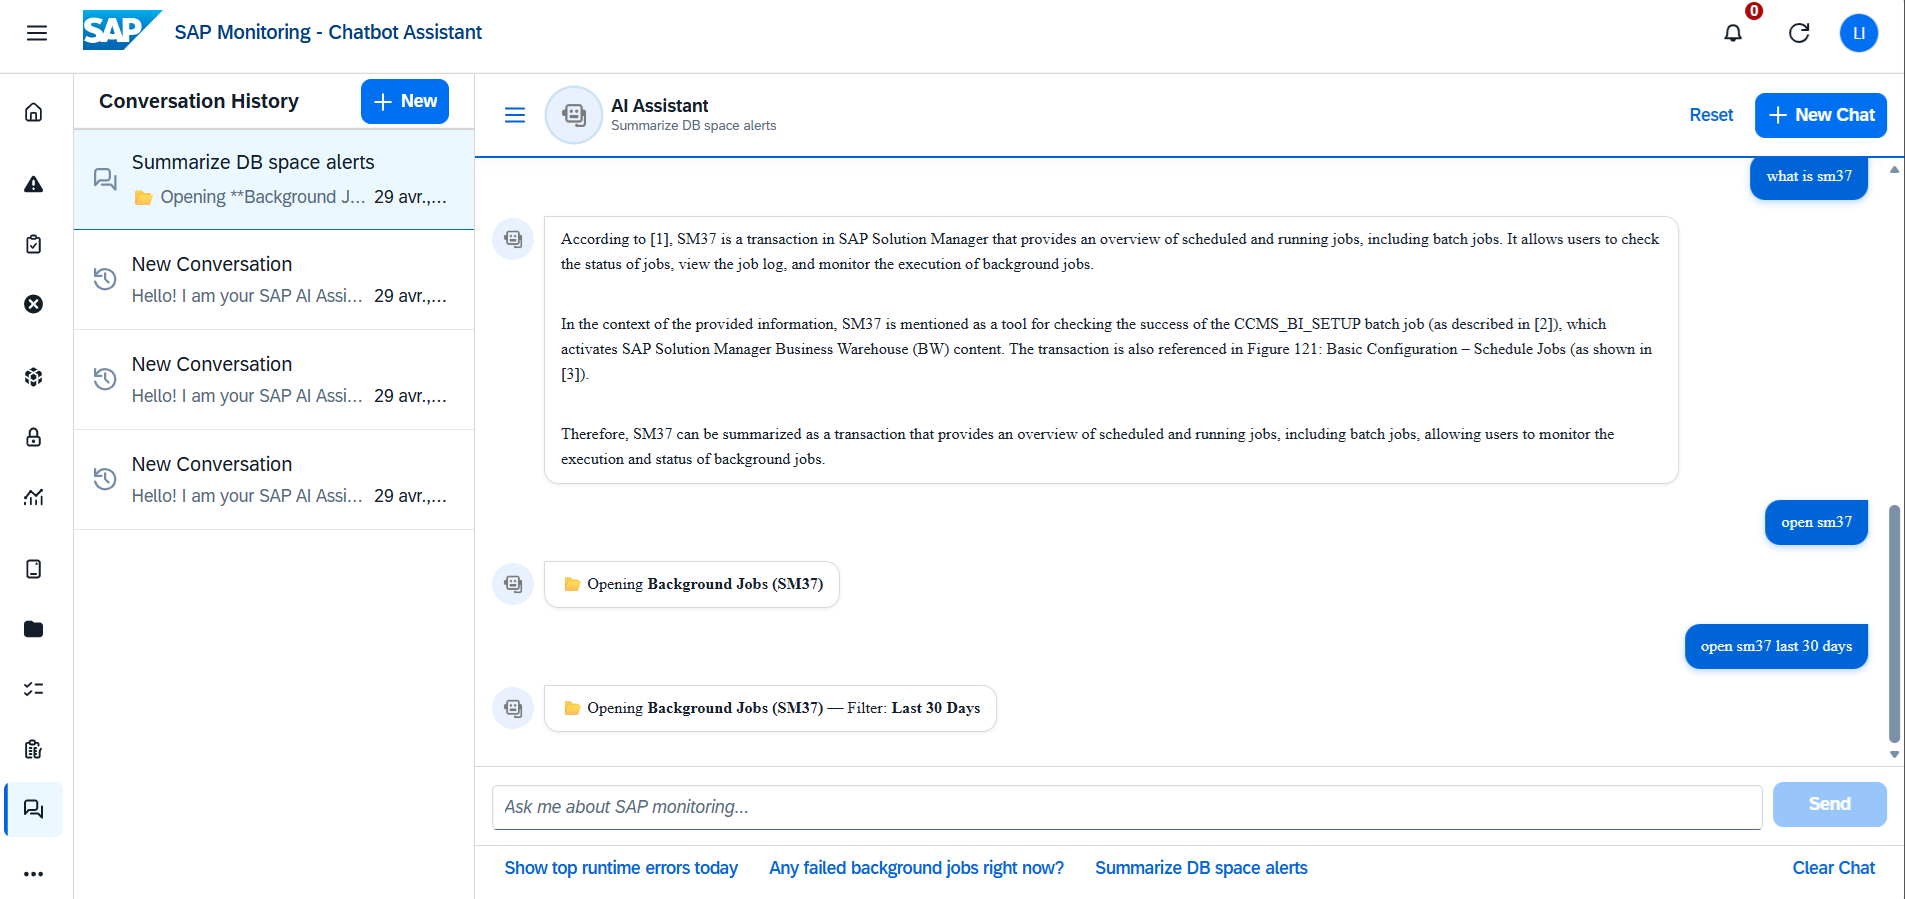
\includegraphics[width=0.9\textwidth]{images/chat.png}
\caption[Interface chatbot avec historique]{Interface de la page chatbot dédiée avec historique de conversations}
\label{fig:chatbot_page}
\end{figure}

\begin{figure}[H]
\centering
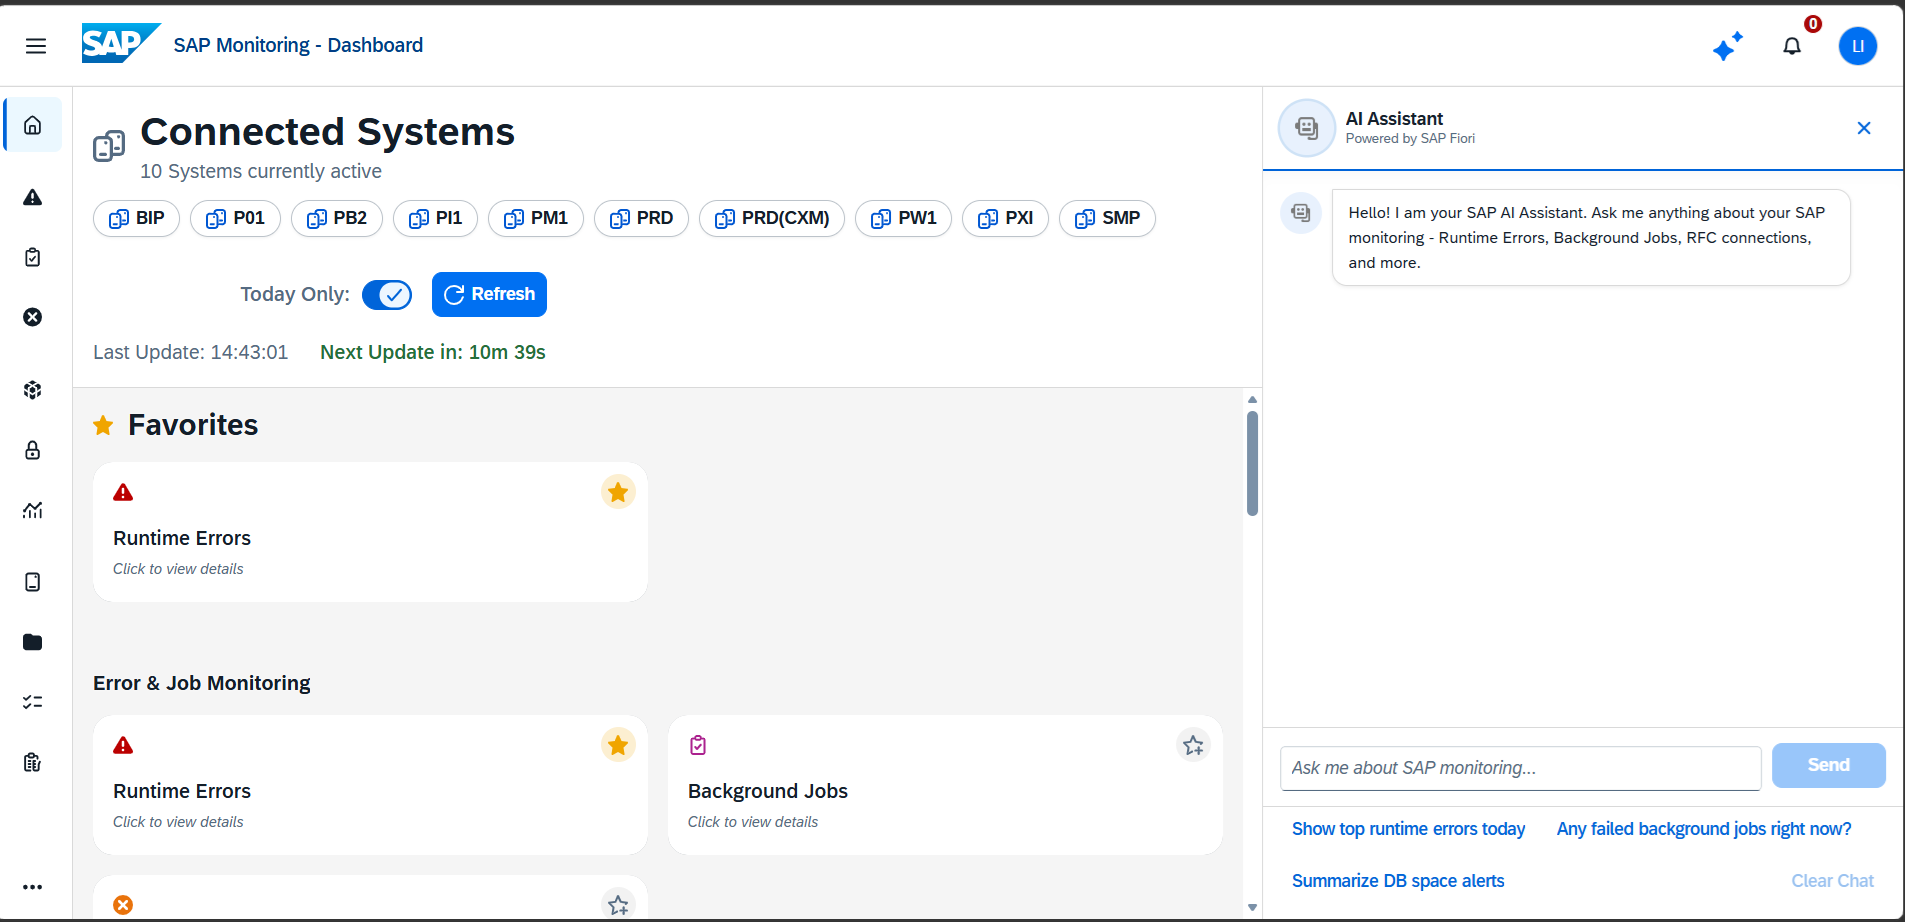
\includegraphics[width=0.9\textwidth]{images/lateral.png}
\caption[ChatPanel en tiroir latéral]{ChatPanel intégré en tiroir latéral sur une page de monitoring SAP}
\label{fig:chatpanel}
\end{figure}

% ─────────────────────────────────────────────────────────────
\section{Sélection du modèle LLM et benchmarking}
% ─────────────────────────────────────────────────────────────

\subsection{Protocole d'évaluation}

Afin de comparer objectivement les deux configurations LLM disponibles, un benchmark automatisé a été conduit le 12 mai 2026. Il porte sur un ensemble de \textbf{10 questions représentatives} des cas d'usage réels du système, couvrant des T-codes BASIS courants~:

\begin{enumerate}[leftmargin=2em]
  \item How to monitor background jobs in SM37?
  \item How to analyze a short dump in ST22?
  \item How to configure transport routes in STMS?
  \item How to manage user roles with SU01 and PFCG?
  \item How to create an ABAP program using SE38?
  \item What is a BAPI and how to test it with SE37?
  \item How to reprocess IDoc errors using BD87?
  \item How to analyze authorization errors with SU53?
  \item How to read system logs in SM21?
  \item How to analyze work processes with SM50?
\end{enumerate}

Les deux modèles évalués sont \textbf{LLaMA~3.2:3b} (modèle rapide, 3 milliards de paramètres) et \textbf{Qwen~2.5:7b} (modèle de qualité supérieure, 7 milliards de paramètres). Les métriques calculées sont le \textbf{Recall@K} (proportion de questions ayant au moins un chunk pertinent dans les K premiers résultats), le \textbf{MRR} (\textit{Mean Reciprocal Rank}, position moyenne du premier chunk pertinent) et le \textbf{nDCG} (\textit{Normalized Discounted Cumulative Gain}, qualité globale du classement). Les valeurs de K testées sont $K \in \{1, 3, 5, 10, 12\}$.

\subsection{Résultats}

La figure~\ref{fig:benchmark} présente les résultats visuels du benchmark comparatif entre les deux configurations LLM sur l'ensemble des métriques de retrieval.

\begin{figure}[H]
\centering
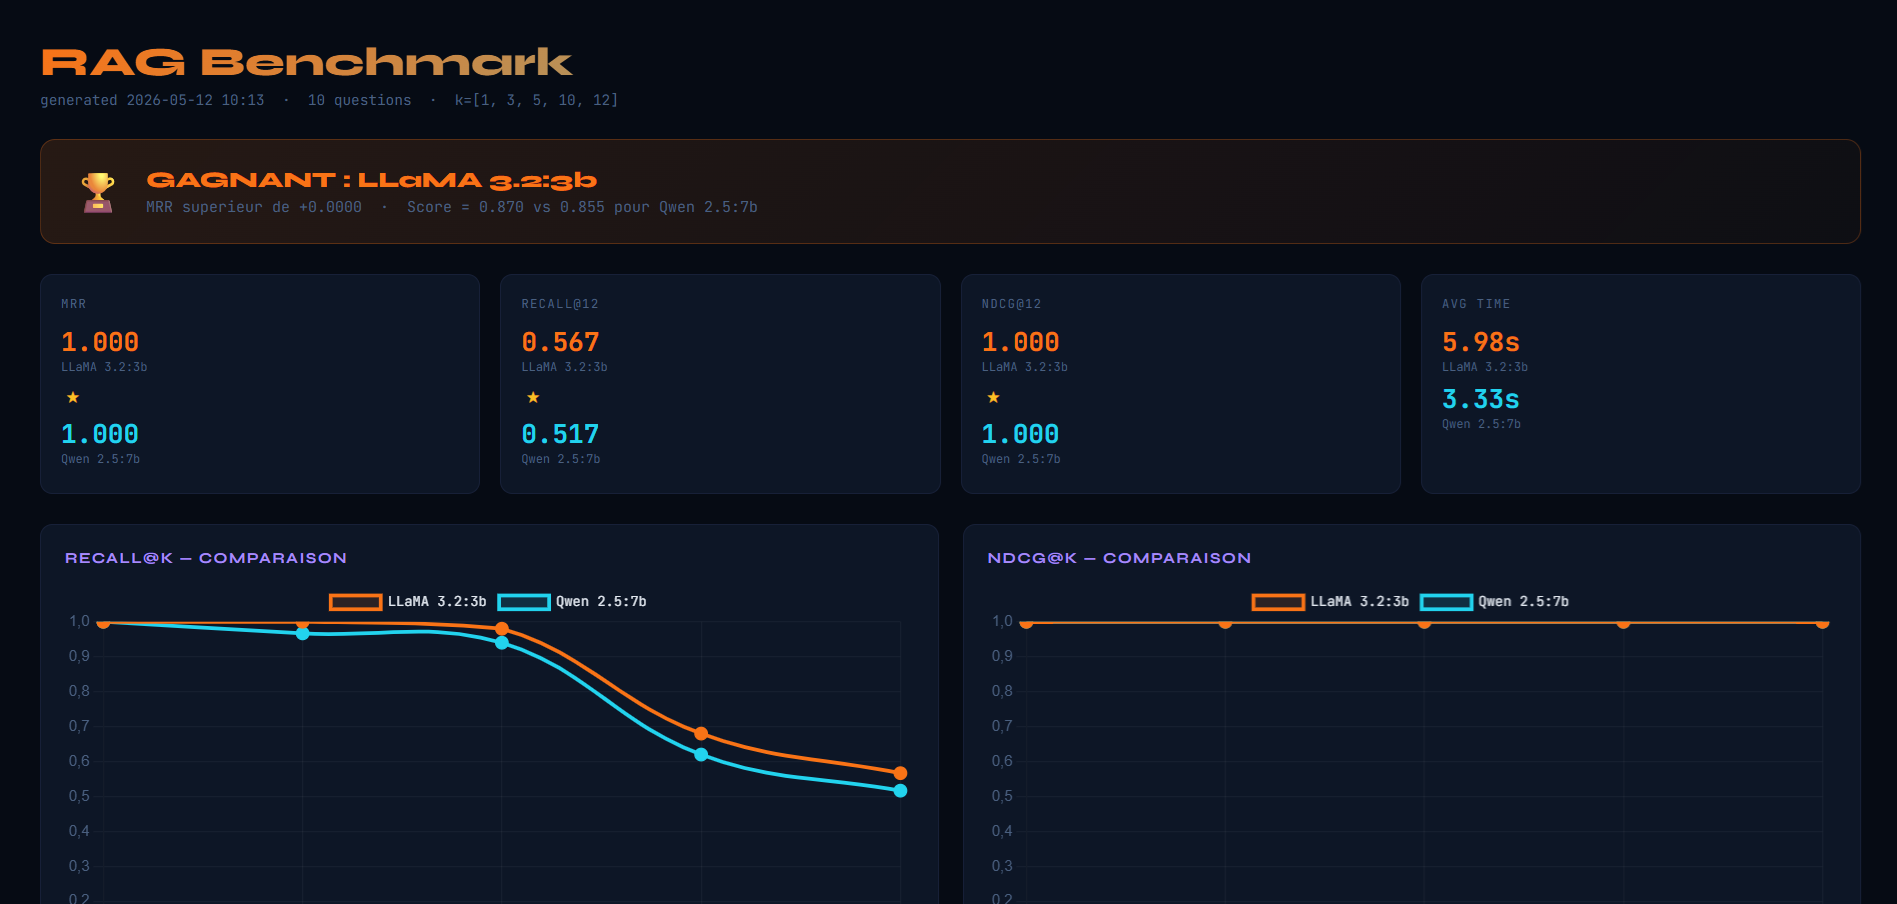
\includegraphics[width=0.95\textwidth]{images/bench.png}
\caption[Benchmark RAG — LLaMA 3.2:3b vs Qwen 2.5:7b]{Résultats du benchmark RAG — LLaMA 3.2:3b vs Qwen 2.5:7b (12 mai 2026, 76~463 vecteurs)}
\label{fig:benchmark}
\end{figure}

\subsection{Analyse des résultats}

Les résultats du benchmark mettent en évidence plusieurs constats~:

\begin{itemize}[leftmargin=2em]
  \item \textbf{Recall@K croissant}~: le rappel augmente logiquement avec K pour les deux modèles, atteignant des valeurs élevées à K=10 et K=12, confirmant que la base documentaire contient les informations nécessaires pour répondre aux questions posées.

  \item \textbf{Qualité de classement}~: le nDCG reflète la capacité du pipeline à placer les chunks les plus pertinents en tête de liste. La fusion RRF avec pondération asymétrique (BM25~: 0.6, vectoriel~: 0.4) favorise la précision lexicale, essentielle pour les T-codes SAP.

  \item \textbf{Impact des paramètres}~: Qwen~2.5:7b utilise un seuil de reranking (\texttt{MIN\_RERANK\_SCORE~=~2.0}) et un \texttt{FETCH\_K~=~40} plus élevés que LLaMA~3.2:3b (\texttt{MIN\_RERANK\_SCORE~=~1.0}, \texttt{FETCH\_K~=~30}), ce qui explique une sélectivité différente dans les résultats.

  \item \textbf{Compromis vitesse/qualité}~: LLaMA~3.2:3b offre des temps de réponse significativement plus courts, tandis que Qwen~2.5:7b produit des réponses de meilleure qualité rédactionnelle. Le choix du modèle peut être configuré dynamiquement via la variable \texttt{model} de la requête API.
\end{itemize}

% ─────────────────────────────────────────────────────────────
\section{Limites et perspectives}
% ─────────────────────────────────────────────────────────────

\subsection{Limites du déploiement actuel}

Malgré les performances satisfaisantes observées lors du benchmark, plusieurs limitations du déploiement actuel méritent d'être soulignées~:

\begin{itemize}[leftmargin=2em]
  \item \textbf{CORS ouvert en développement}~: La politique CORS de l'API FastAPI est actuellement configurée en mode permissif (\texttt{allow\_origins=["*"]}), adapté à un environnement de développement. Une configuration restrictive sera nécessaire pour un déploiement en production.

  \item \textbf{Cache sémantique en mémoire}~: Le cache sémantique du pipeline RAG est stocké uniquement en mémoire vive du processus. Son contenu est perdu à chaque redémarrage et ne peut pas être partagé entre plusieurs instances, ce qui limite son efficacité dans une architecture distribuée.

  \item \textbf{LLM local limité}~: Le modèle \texttt{llama3.2:3b} déployé localement via Ollama, bien qu'adapté à un contexte \textit{on-premise}, reste moins performant que les grands modèles hébergés dans le cloud (GPT-4o, Claude Sonnet) sur des questions complexes nécessitant un raisonnement approfondi.

  \item \textbf{Gestion des sessions en mémoire}~: Les sessions de conversation de l'API FastAPI sont stockées dans un dictionnaire Python en mémoire. En cas de redémarrage du service, toutes les sessions actives sont perdues. La persistance des sessions dans la base de données PostgreSQL est déjà implémentée mais dépend d'un mécanisme asynchrone de sauvegarde.

  \item \textbf{Détection d'hallucinations par heuristiques}~: La validation anti-hallucination repose sur des expressions régulières pour les T-codes et les numéros de notes SAP. Les affirmations factuellement erronées ne contenant pas d'identifiants SAP explicites ne sont pas détectées.
\end{itemize}

\subsection{Perspectives d'amélioration}

Plusieurs axes d'amélioration peuvent être envisagés pour renforcer le système à court et moyen terme~:

\begin{itemize}[leftmargin=2em]
  \item \textbf{Déploiement Cloud Foundry}~: Les fichiers \texttt{mta.yaml} et \texttt{manifest.yml} sont déjà configurés pour un déploiement sur SAP BTP (\textit{Business Technology Platform}) via Cloud Foundry. Cette étape permettrait de bénéficier d'une haute disponibilité, d'un équilibrage de charge et d'une authentification XSUAA intégrée.

  \item \textbf{Cache sémantique distribué}~: L'intégration d'un cache Redis permettrait de partager le cache sémantique entre plusieurs instances de l'API RAG et de le persister entre les redémarrages.

  \item \textbf{Modèle LLM plus performant}~: L'intégration d'un modèle de grande taille (qwen2.5:7b déjà supporté, ou un modèle cloud via API) améliorerait la qualité des réponses sur les requêtes complexes.

  \item \textbf{Mise à jour incrémentale de la base de connaissances}~: Un pipeline de synchronisation incrémentale (déjà prototypé dans \texttt{conv\_databaseMONGODB/}) permettrait d'enrichir automatiquement la base documentaire à mesure que de nouvelles notes SAP ou documentations sont publiées.

  \item \textbf{Collecte de feedback utilisateur}~: L'ajout d'un mécanisme de notation des réponses (pouce haut/pouce bas) permettrait de constituer un jeu de données d'évaluation continue et d'identifier les points faibles du système en production réelle.
\end{itemize}

% ─────────────────────────────────────────────────────────────
\section*{Conclusion}
% ─────────────────────────────────────────────────────────────
Ce chapitre a présenté le déploiement complet du système RAG SAP dans le cadre de la méthodologie CRISP-DM. L’architecture développée repose sur trois couches complémentaires : un backend Python/FastAPI pour le moteur RAG, un service SAP CAP assurant l’exposition OData, et une interface React SAP UI5 intégrant le chatbot. Les résultats du benchmark ont confirmé l’efficacité du pipeline hybride de retrieval sur un corpus SAP volumineux de 76~463 vecteurs. En environnement de production, la solution permet aux administrateurs SAP BASIS d’obtenir rapidement des réponses techniques fiables directement depuis l’interface de monitoring. Enfin, les perspectives d’évolution, notamment l’intégration sur SAP BTP et l’utilisation de modèles LLM plus performants, ouvrent la voie à une industrialisation avancée de la plateforme.